
\documentclass[letterpaper,hide notes,xcolor={table,svgnames},pdftex,10pt]{beamer}
\def\showexamples{t}

\usecolortheme{crane}
\setbeamertemplate{navigation symbols}{}

\usetheme{MyPittsburgh}
\usepackage{hyperref}
\usepackage{graphicx,xspace}
\usepackage[normalem]{ulem}
\usepackage{multicol}
\usepackage{amsmath,amssymb,amsthm,graphicx,xspace}
\newcommand\SF[1]{$\bigstar$\footnote{SF: #1}}

\usepackage[sfdefault,lf]{carlito}
\usepackage[T1]{fontenc}
\usepackage[scaled]{beramono}
\usepackage{tikzpagenodes}
\newcommand{\Rplus}{\protect\hspace{-.1em}\protect\raisebox{.35ex}{\small{\small\textbf{+}}}}
\newcommand{\Cpp}{\mbox{C\Rplus\Rplus}\xspace}

\newcounter{tmpnumSlide}
\newcounter{tmpnumNote}

\newcommand\mnote[1]{%
	\addtocounter{tmpnumSlide}{1}
	\ifdefined\showcues {~\tiny\fbox{\arabic{tmpnumSlide}}}\fi
	\note{\setlength{\parskip}{1ex}\addtocounter{tmpnumNote}{1}\textbf{\Large \arabic{tmpnumNote}:} {#1\par}}}

\newcommand\mmnote[1]{\note{\setlength{\parskip}{1ex}#1\par}}


\newcommand\mquestion[2]{{~\color{red}\fbox{?}}\note{\setlength{\parskip}{1ex}\par{\Large \textbf{?}} #1} \note{\setlength{\parskip}{1ex}\par{\Large \textbf{A}} #2\par}\ifdefined \presentationonly \pause \fi}

\newcommand\blackboard[1]{%
	\ifdefined   \showblackboard
		{#1}
	\else {\begin{center} \fbox{\colorbox{blue!30}{%
						\begin{minipage}{.95\linewidth}%
							\hspace{\stretch{1}} Some space intentionally left blank; done at the blackboard.%
						\end{minipage}}}\end{center}}%
	\fi%
}

\usepackage{listings}
\lstset{%
	keywordstyle=\bfseries,
	aboveskip=15pt,
	belowskip=15pt,
	captionpos=b,
	identifierstyle=\ttfamily,
	frame=lines,
	numbers=left, basicstyle=\scriptsize, numberstyle=\tiny, stepnumber=0, numbersep=2pt}

\usepackage{siunitx}
\newcommand\sius[1]{\num[group-separator = {,}]{#1}\si{\micro\second}}
\newcommand\sims[1]{\num[group-separator = {,}]{#1}\si{\milli\second}}
\newcommand\sins[1]{\num[group-separator = {,}]{#1}\si{\nano\second}}
\sisetup{group-separator = {,}, group-digits = true}

%% -------------------- tikz --------------------
\usepackage{tikz}
\usetikzlibrary{positioning}
\usetikzlibrary{arrows,backgrounds,automata,decorations.shapes,decorations.pathmorphing,decorations.markings,decorations.text}

\tikzstyle{place}=[circle,draw=blue!50,fill=blue!20,thick, inner sep=0pt,minimum size=6mm]
\tikzstyle{transition}=[rectangle,draw=black!50,fill=black!20,thick, inner sep=0pt,minimum size=4mm]

\tikzstyle{block}=[rectangle,draw=black, thick, inner sep=5pt]
\tikzstyle{bullet}=[circle,draw=black, fill=black, thin, inner sep=2pt]

\tikzstyle{pre}=[<-,shorten <=1pt,>=stealth',semithick]
\tikzstyle{post}=[->,shorten >=1pt,>=stealth',semithick]
\tikzstyle{bi}=[<->,shorten >=1pt,shorten <=1pt, >=stealth',semithick]

\tikzstyle{mut}=[-,>=stealth',semithick]

\tikzstyle{treereset}=[dashed,->, shorten >=1pt,>=stealth',thin]

\usepackage{ifmtarg}
\usepackage{xifthen}
\makeatletter
% new counter to now which frame it is within the sequence
\newcounter{multiframecounter}
% initialize buffer for previously used frame title
\gdef\lastframetitle{\textit{undefined}}
% new environment for a multi-frame
\newenvironment{multiframe}[1][]{%
	\ifthenelse{\isempty{#1}}{%
		% if no frame title was set via optional parameter,
		% only increase sequence counter by 1
		\addtocounter{multiframecounter}{1}%
	}{%
		% new frame title has been provided, thus
		% reset sequence counter to 1 and buffer frame title for later use
		\setcounter{multiframecounter}{1}%
		\gdef\lastframetitle{#1}%
	}%
	% start conventional frame environment and
	% automatically set frame title followed by sequence counter
	\begin{frame}%
		\frametitle{\lastframetitle~{\normalfont(\arabic{multiframecounter})}}%
		}{%
	\end{frame}%
}
\makeatother

\makeatletter
\newdimen\tu@tmpa%
\newdimen\ydiffl%
\newdimen\xdiffl%
\newcommand\ydiff[2]{%
	\coordinate (tmpnamea) at (#1);%
	\coordinate (tmpnameb) at (#2);%
	\pgfextracty{\tu@tmpa}{\pgfpointanchor{tmpnamea}{center}}%
	\pgfextracty{\ydiffl}{\pgfpointanchor{tmpnameb}{center}}%
	\advance\ydiffl by -\tu@tmpa%
}
\newcommand\xdiff[2]{%
	\coordinate (tmpnamea) at (#1);%
	\coordinate (tmpnameb) at (#2);%
	\pgfextractx{\tu@tmpa}{\pgfpointanchor{tmpnamea}{center}}%
	\pgfextractx{\xdiffl}{\pgfpointanchor{tmpnameb}{center}}%
	\advance\xdiffl by -\tu@tmpa%
}
\makeatother
\newcommand{\copyrightbox}[3][r]{%
	\begin{tikzpicture}%
		\node[inner sep=0pt,minimum size=2em](ciimage){#2};
		\usefont{OT1}{phv}{n}{n}\fontsize{4}{4}\selectfont
		\ydiff{ciimage.south}{ciimage.north}
		\xdiff{ciimage.west}{ciimage.east}
		\ifthenelse{\equal{#1}{r}}{%
			\node[inner sep=0pt,right=1ex of ciimage.south east,anchor=north west,rotate=90]%
			{\raggedleft\color{black!50}\parbox{\the\ydiffl}{\raggedright{}#3}};%
		}{%
			\ifthenelse{\equal{#1}{l}}{%
				\node[inner sep=0pt,right=1ex of ciimage.south west,anchor=south west,rotate=90]%
				{\raggedleft\color{black!50}\parbox{\the\ydiffl}{\raggedright{}#3}};%
			}{%
				\node[inner sep=0pt,below=1ex of ciimage.south west,anchor=north west]%
				{\raggedleft\color{black!50}\parbox{\the\xdiffl}{\raggedright{}#3}};%
			}
		}
	\end{tikzpicture}
}


%% --------------------

%\usepackage[excludeor]{everyhook}
%\PushPreHook{par}{\setbox0=\lastbox\llap{MUH}}\box0}

%\vspace*{\stretch{1}

%\setbox0=\lastbox \llap{\textbullet\enskip}\box0}

\setlength{\parskip}{\fill}

\newcommand\noskips{\setlength{\parskip}{1ex}}
\newcommand\doskips{\setlength{\parskip}{\fill}}

\newcommand\xx{\par\vspace*{\stretch{1}}\par}
\newcommand\xxs{\par\vspace*{2ex}\par}
\newcommand\tuple[1]{\langle #1 \rangle}
\newcommand\code[1]{{\sf \footnotesize #1}}
\newcommand\ex[1]{\uline{Example:} \ifdefined \presentationonly \pause \fi
	\ifdefined\showexamples#1\xspace\else{\uline{\hspace*{2cm}}}\fi}

\newcommand\ceil[1]{\lceil #1 \rceil}


\AtBeginSection[]
{
	\begin{frame}
		\frametitle{Outline}
		\tableofcontents[currentsection]
	\end{frame}
}



\pgfdeclarelayer{edgelayer}
\pgfdeclarelayer{nodelayer}
\pgfsetlayers{edgelayer,nodelayer,main}

\tikzstyle{none}=[inner sep=0pt]
\tikzstyle{rn}=[circle,fill=Red,draw=Black,line width=0.8 pt]
\tikzstyle{gn}=[circle,fill=Lime,draw=Black,line width=0.8 pt]
\tikzstyle{yn}=[circle,fill=Yellow,draw=Black,line width=0.8 pt]
\tikzstyle{empty}=[circle,fill=White,draw=Black]
\tikzstyle{bw} = [rectangle, draw, fill=blue!20,
text width=4em, text centered, rounded corners, minimum height=2em]

\newcommand{\CcNote}[1]{% longname
	This work is licensed under the \textit{Creative Commons #1 3.0 License}.%
}
\newcommand{\CcImageBy}[1]{%
	\includegraphics[scale=#1]{creative_commons/cc_by_30.pdf}%
}
\newcommand{\CcImageSa}[1]{%
	\includegraphics[scale=#1]{creative_commons/cc_sa_30.pdf}%
}
\newcommand{\CcImageNc}[1]{%
	\includegraphics[scale=#1]{creative_commons/cc_nc_30.pdf}%
}
\newcommand{\CcGroupBySa}[2]{% zoom, gap
	\CcImageBy{#1}\hspace*{#2}\CcImageNc{#1}\hspace*{#2}\CcImageSa{#1}%
}
\newcommand{\CcLongnameByNcSa}{Attribution-NonCommercial-ShareAlike}

\newenvironment{changemargin}[1]{% 
	\begin{list}{}{% 
		\setlength{\topsep}{0pt}% 
		\setlength{\leftmargin}{#1}% 
		\setlength{\rightmargin}{1em}
		\setlength{\listparindent}{\parindent}% 
		\setlength{\itemindent}{\parindent}% 
		      \setlength{\parsep}{\parskip}% 
		      }% 
		\item[]}{\end{list}}




\title{Lecture 17 --- Scheduling Algorithm Evaluation; UNIX \& Windows}

\author{Jeff Zarnett \\ \small \texttt{jzarnett@uwaterloo.ca}}
\institute{Department of Electrical and Computer Engineering \\
  University of Waterloo}
\date{\today}


\begin{document}

\begin{frame}
  \titlepage

 \end{frame}
 
\part{Algorithm Evaluation}

\begin{frame}
\partpage
\end{frame}
 
\begin{frame}
\frametitle{What Do We Choose?}

In some cases (real-time?) it's obvious what to choose.

Otherwise, what gives the best overall performance?

This requires a clear definition of best...\\
\quad Let's assume we have one.

\end{frame}

\begin{frame}
\frametitle{How to Decide?}

We need to evaluate the algorithms we've discussed in terms of how well they achieve that goal. 

While it is possible to just have a theoretical discussion about it where we say we think $A$ is better than $B$ but worse than $C$, that's not a very scientific approach. 

What we'd like to do instead is gather some data and make the decision using it.

\end{frame}

\begin{frame}
\frametitle{Deterministic Modelling}

Looks like writing test scenarios for a lab project.

Test scenario has inputs/outputs and check correctness/performance.

\end{frame}

\begin{frame}
\frametitle{Deterministic Modelling}

An example of a simple test case looks like this, where all five processes arrive at time 0 in this order:

\begin{center}
\begin{tabular}{c|r}
	\textbf{Process ID} & \textbf{Burst Time}\\ \hline
	1 & 10 \\
	2 & 29 \\
	3 & 3 \\
	4 & 7 \\
	5 & 12 \\
\end{tabular}
\end{center}

Then run the target scheduling algorithms.

\end{frame}

\begin{frame}
\frametitle{Deterministic Modelling}

Wait times:

FCFS: 28\\
SJF: 13\\
RR(10): 23

Total time of execution is the same... right?

\end{frame}

\begin{frame}
\frametitle{Process Switch Penalty}

\begin{center}
	
\includegraphics[width=0.4\textwidth]{images/free-realestate.jpg}
\end{center}

A more precise version of this evaluation would assign a penalty to the process switch.

\end{frame}


\begin{frame}
\frametitle{Context Switches}

FCFS and SJF have 4 switches; RR has 7.

Maybe context switch time is so small as to be irrelevant?

\end{frame}

\begin{frame}
\frametitle{More Realistic}

Test cases that look more realistic will not have everything be statically initialized at the beginning and all tasks waiting.

\begin{center}
	
\includegraphics[width=0.5\textwidth]{images/simulations.jpg}
\end{center}

The nice thing about the deterministic modelling approach is that the tests are reproducible and produce consistent results on every run.

\end{frame}

\begin{frame}
\frametitle{Oh no, Math}

The real behaviour of most systems looks very different from how the deterministic approach models it.

\begin{center}
	
\includegraphics[width=0.6\textwidth]{images/dnd.jpg}
\end{center}

Real systems have a lot of randomness in them...

\end{frame}

\begin{frame}
\frametitle{Queueing Theory}

Example: login times are somewhat random, but not totally.

That leads us to queueing theory.

\begin{center}
	
\includegraphics[width=0.4\textwidth]{images/math.jpg}
\end{center}

That's too advanced for this course.

\end{frame}

\begin{frame}
\frametitle{Simulations and Emulation}

The simulation, if designed appropriately, will account for more things like clock interrupts and context switch times.

It's possible to do an all-software simulation...

The simulation is only as accurate as you make it and there are a lot of things that might be difficult to simulate accurately.

\end{frame}

\begin{frame}
\frametitle{Embedded Platform?}

Your system may come with an emulator that saves you a lot of work!

\begin{center}
	
\includegraphics[width=0.4\textwidth]{images/emulator.jpg}
\end{center}

\end{frame}

\begin{frame}
\frametitle{Simulation Limitation}

Simulations are always based on some assumptions.

A general purpose OS also needs to work for many different HW configurations...

Actually, let's consider some real OS algorithms.

\end{frame}


\part{Windows \& UNIX Scheduling}

\begin{frame}
\partpage
\end{frame}

\begin{frame}
\frametitle{Scheduling in Desktop OSes}

In this lecture we will examine how real commercial operating systems schedule their processes and threads. 

We will examine UNIX and Windows scheduling. 

We will see what approaches are used and what is interesting/novel about them.


\end{frame}

\begin{frame}
\frametitle{Traditional UNIX}

The traditional UNIX scheduling is really ancient; as in System V R3 and BSD 4.3.\\
\quad It was replaced in SVR4 (which had some real-time support).

Multilevel feedback system using Round Robin within each of the queues. 

Time slicing is implemented and the default time slice is a (very long) 1 second. 

So if a process does not block or complete within 1~s, then it will be preempted. 

Priority is based on the process type as well as the execution history.

\end{frame}

\begin{frame}
\frametitle{Traditional UNIX}

Processor utilization for a process $j$ is calculated for an interval $i$ as:

\begin{center}
$CPU_{j}(i) = \dfrac{CPU_{j}(i - 1)}{2}$
\end{center}

And the priority is for process $j$ at interval $i$ is calculated by the formula:

\begin{center}
$P_{j}(i) = B_{j} + \dfrac{CPU_{j}}{2} + N_{j}$
\end{center}

where $B_{j}$ is the base priority of process $j$ and $N_{j}$ is the ``nice'' value of process $j$.


\end{frame}

\begin{frame}
\frametitle{Be Nice}

The ``nice'' value is a UNIX way to allow a user to voluntarily reduce the priority of a process to be ``nice'' to other users (but honestly, who uses this?).

Actually, the answer to that question is: system administrators. 

An admin can ``re-nice'' a process and make it somewhat nicer than it would otherwise be.


\end{frame}

\begin{frame}
\frametitle{Traditional UNIX}

The $CPU$ and $N$ components of the equation are restricted to prevent a process from migrating outside of its assigned category. 

A process is assigned to a given category based on what kind of process it is. 

To put it in simple terms, the OS puts its own needs first and tries to make the best use of resources it can.


\end{frame}

\begin{frame}
\frametitle{Traditional UNIX}

From highest to lowest priority, the categories are:

\begin{enumerate}
	\item Swapper (move processes to and from disk)
	\item Block I/O device control (e.g., disk)
	\item File manipulation
	\item Character I/O device control (e.g., keyboard)
	\item User processes
\end{enumerate}



\end{frame}

\begin{frame}
\frametitle{Traditional UNIX}

Yes, unfortunately, user processes get piled at the bottom of the list. 

It should provide for efficient use of I/O devices and tends to penalize processor-bound processes at the expense of I/O bound processes. 

CPU-bound processes should be able to carry on executing when an I/O-bound process waits for the I/O operation to complete. 

When an I/O operation is finished, we would like to start the next I/O operation so the I/O device is not waiting.

This strategy is reasonably effective for a general-purpose, time-sharing operating system.

\end{frame}

\begin{frame}
\frametitle{Upgrading to SVR4}

SRV4: highest priority to real-time, then kernel, then user-mode.

Big differences are:\\
\quad (1) more priority levels -- 160 broken down into three types\\
\quad (2) preemption points

Preemption points were needed!

\end{frame}

\begin{frame}
\frametitle{FreeBSD}
FreedBSD has a scheduling process that's quite similar to that of SRV4.

Interactivity scoring mechanism: which are user-interactive?

\end{frame}

\begin{frame}
\frametitle{Scoring Mechanism}

We'll define the maximum interactivity score as $m$, the runtime of the thread as $r$ and the sleep time of the thread as $s$. 

More sleep time than run time? The interactivity score is calculated as $(\dfrac{m}{2})(\dfrac{r}{s})$

For those that have more run time than sleep time:
  $(\dfrac{m}{2})(1 + \dfrac{r}{s})$. 

\end{frame}

\begin{frame}
\frametitle{Affinity and Load-Balancing}

We already covered affinity and load-balancing.

FreeBSD has push and pull mechanisms.

Pull: bit mask to indicate it's idle.

Push: Twice per second tasks to equalize highest and lowest CPUs.


\end{frame}

\begin{frame}
\frametitle{Windows Scheduling}

Windows schedules threads using a priority-based, preemptive scheduling algorithm, ensuring that the highest priority thread runs. 

The official name for the selection routine is the \alert{dispatcher}.

A thread runs until it is preempted, blocks, terminates, or its time slice expires. 

\end{frame}

\begin{frame}
\frametitle{Windows Scheduling}

If a higher priority thread is unblocked, it will preempt a lower priority thread. 

Windows has 32 different priority levels, the regular (priority 1 to 15) and real-time classes (16 to 31). 

A memory management task runs at priority 0.

The dispatcher maintains a queue for each of the scheduling priorities and goes through them from highest to lowest until it finds something to do.

If there is nothing else currently ready, the System Idle Process will ``run''.

\end{frame}

\begin{frame}
\frametitle{Windows Priority Classes}

There are six priority classes you can set a process to via Task Manager:

\begin{enumerate}
	\item Realtime
	\item High
	\item Above Normal
	\item Normal
	\item Below Normal
	\item Low
\end{enumerate}

A process is usually in the Normal class.

\end{frame}

\begin{frame}
\frametitle{Windows Thread Priorities}

\begin{center}
	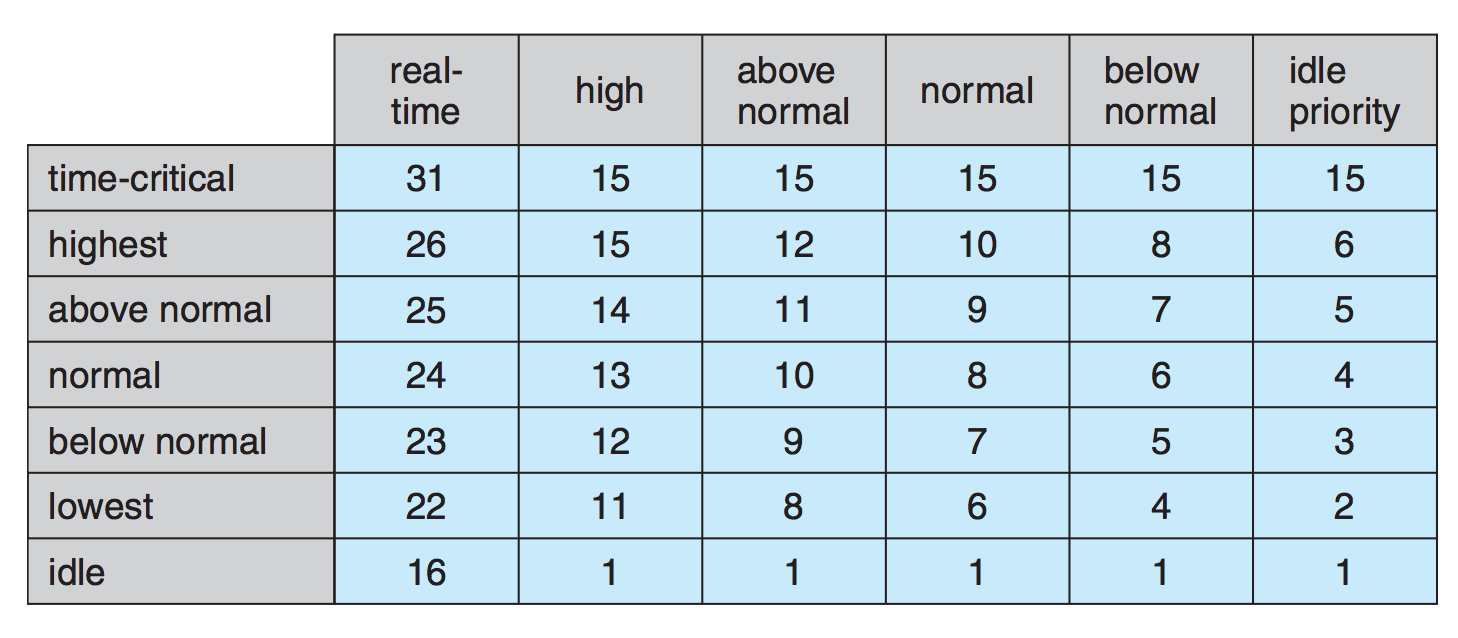
\includegraphics[width=\textwidth]{images/windows-thread-priorities.png}
\end{center}

\end{frame}

\begin{frame}
\frametitle{Windows Time Slicing}

If a process reaches the end of a time slice, the thread is interrupted.

Unless it is in the real-time category, its priority will be lowered, to a minimum of the base priority of each class. 

When a process that was blocked on something (e.g., a wait or I/O), its priority is temporarily boosted (unless it is real-time, in which case it cannot be boosted). 

The amount of the boost depends on what the event was.

A process that was waiting for keyboard input gets a bigger boost than one that was waiting for a disk operation, for example.

\end{frame}

\begin{frame}
\frametitle{Windows Priority: UI}

The operating system also gives a priority to whatever process is running in the selected foreground window. 

This is different from foreground vs. background processes, because the definition of a foreground process was one that was user-interactive. 

Here, the distinction is which of the user-interactive processes is currently ``on top'' in the UI. 

Not only does this process get a priority boost, but it also gets longer time slices. 

It highlights the different heritages of Windows and UNIX...

\end{frame}



\end{document}

